%\begin{savequote}[8cm]
%\textlatin{Cor animalium, fundamentum e\longs t vitæ, princeps omnium, Microco\longs mi Sol, a quo omnis vegetatio dependet, vigor omnis \& robur emanat.}

%The heart of animals is the foundation of their life, the sovereign of everything within them, the sun of their microcosm, that upon which all growth depends, from which all power proceeds.
 % \qauthor{--- William Harvey \cite{harvey_exercitatio_1628}}
%\end{savequote}

\chapter{Experiment photos and equipment list} \label{app:experimentphotos}

\minitoc

This appendix contains a detailed description of the experiment. A table is given with a full description of the key optics used in the experiment. Then, a series of photographs are provided showing different aspects of the experiment setup. Full CAD models and technical drawings (provided by the CLF CAD team) are also displayed.

\section{Final experimental results}

Table \ref{tab:Data table} provides the key experimental data for each of the shots in the final data set.

%\begin{landscape}
	\begin{table*}
		\caption{\label{tab:Data table} Principal Hugoniot data for the compressed foam. $U_s^{quartz}$ and $U_s^{foam}$ are the measured quartz and foam shock velocities. The quartz particle velocity, pressure, and temperature ($u_p^{quartz}$, $P^{quartz}$ and $T^{quartz}$) are not directly measured, and are instead calculated from the shock velocity using known relations (the  Hugoniot \cite{Knudson2013}, and a measured relationship between $U_s^{quartz}$ and $T^{quartz}$ \cite{Millot2015}). $u_p^{foam}$ and $P^{foam}$ are the foam particle velocity and pressure, determined from the impedance matching calculation, while $T^{foam}$ is the foam grey-body temperature calculated in the SOP analysis. Other than $U_s^{quartz}$ and $U_s^{foam}$, where the quoted error is the experimental uncertainty, the errors given for each value are the standard deviation of a distribution for that value obtained from 10,000 random Monte-Carlo iterations. The SOP did not work correctly on all shots, hence the missing $T^{foam}$ values. }
		
		\renewcommand{\arraystretch}{1.35}
		\resizebox{\textwidth}{!}{%
			\begin{tabular}{ccccccccc}
				\hline\hline
				$U_s^{quartz}$ (\si[per-mode=symbol]{km/s}) & $u_p^{quartz}$ (\si[per-mode=symbol]{km/s}) & $P^{quartz}$ (\si[per-mode=symbol]{GPa}) & $T^{quartz}$ (\si[per-mode=symbol]{eV}) & $U_s^{foam}$ (\si[per-mode=symbol]{km/s}) & $u_p^{foam}$ (\si[per-mode=symbol]{km/s})  &$P^{foam}$ (\si[per-mode=symbol]{GPa}) &  $T^{foam}$ (\si[per-mode=symbol]{eV}) \\ \hline
				$9.2	\pm  0.6 $	& $4.3\ 	^{+\ 0.4}	_{-\ 0.4}$	& $106 \ 	^{+\ 17}	_{-\ 16} $	& -			& $11.1	\pm  1.1 $	& $6.8\ 	^{+\ 0.6}	_{-\ 0.7}$	& $19.2\ 	^{+\ 3.0}	_{-\ 2.1}$	& -			\\
				$13.4	\pm  2.4 $	& $7.0\ 	^{+\ 1.8}	_{-\ 1.6}$	& $249 \ 	^{+\ 123}	_{-\ 93} $	& $0.96\ 	^{+\ 0.59}	_{-\ 0.40}$	& $15.9	\pm  4.9 $	& $11.1\ 	^{+\ 3.2}	_{-\ 2.8}$	& $44.4\ 	^{+\ 19.3}	_{-\ 16.0}$	& $0.60\ 	^{+\ 0.30}	_{-\ 0.23}$	\\
				$13.4	\pm  0.4 $	& $7.0\ 	^{+\ 0.2}	_{-\ 0.2}$	& $250 \ 	^{+\ 16}	_{-\ 15} $	& -			& $22.3	\pm  3.5 $	& $10.5\ 	^{+\ 0.5}	_{-\ 0.5}$	& $59.0\ 	^{+\ 9.9}	_{-\ 7.3}$	& -			\\
				$13.5	\pm  1.0 $	& $7.1\ 	^{+\ 0.7}	_{-\ 0.7}$	& $253 \ 	^{+\ 47}	_{-\ 42} $	& $0.98\ 	^{+\ 0.21}	_{-\ 0.18}$	& $17.0	\pm  2.0 $	& $11.0\ 	^{+\ 1.2}	_{-\ 1.2}$	& $47.4\ 	^{+\ 8.6}	_{-\ 6.2}$	& $0.62\ 	^{+\ 0.16}	_{-\ 0.13}$	\\
				$14.3	\pm  1.5 $	& $7.7\ 	^{+\ 1.0}	_{-\ 1.0}$	& $290 \ 	^{+\ 73}	_{-\ 64} $	& $1.14\ 	^{+\ 0.35}	_{-\ 0.28}$	& $16.3	\pm  2.7 $	& $12.1\ 	^{+\ 1.9}	_{-\ 1.8}$	& $50.0\ 	^{+\ 12.0}	_{-\ 9.4}$	& $0.68\ 	^{+\ 0.20}	_{-\ 0.17}$	\\
				$14.4	\pm  2.7 $	& $7.7\ 	^{+\ 2.0}	_{-\ 1.9}$	& $296 \ 	^{+\ 150}	_{-\ 117} $	& $1.17\ 	^{+\ 0.76}	_{-\ 0.53}$	& $14.5	\pm  3.3 $	& $12.5\ 	^{+\ 3.7}	_{-\ 3.3}$	& $45.7\ 	^{+\ 17.9}	_{-\ 14.8}$	& $0.69\ 	^{+\ 0.35}	_{-\ 0.28}$	\\
				$15.7	\pm  1.8 $	& $8.7\ 	^{+\ 1.3}	_{-\ 1.2}$	& $362 \ 	^{+\ 102}	_{-\ 87} $	& -			& $25.2	\pm  2.8 $	& $13.0\ 	^{+\ 2.2}	_{-\ 2.1}$	& $82.9\ 	^{+\ 18.8}	_{-\ 13.9}$	& -			\\
				$16.9	\pm  1.1 $	& $9.5\ 	^{+\ 0.8}	_{-\ 0.8}$	& $423 \ 	^{+\ 69}	_{-\ 62} $	& $1.79\ 	^{+\ 0.36}	_{-\ 0.31}$	& $19.0	\pm  2.5 $	& $15.1\ 	^{+\ 1.5}	_{-\ 1.5}$	& $72.3\ 	^{+\ 13.2}	_{-\ 9.6}$	& $1.29\ 	^{+\ 0.31}	_{-\ 0.24}$	\\
				$21.6	\pm  0.8 $	& $13.1\ 	^{+\ 0.7}	_{-\ 0.7}$	& $749 \ 	^{+\ 69}	_{-\ 66} $	& $3.62\ 	^{+\ 0.42}	_{-\ 0.40}$	& $22.3	\pm  2.3 $	& $21.2\ 	^{+\ 1.2}	_{-\ 1.4}$	& $120.0\ 	^{+\ 16.1}	_{-\ 10.9}$	& $1.43\ 	^{+\ 0.32}	_{-\ 0.26}$	\\
				\hline\hline
		\end{tabular}}
	\end{table*}
%\end{landscape}





\begin{landscape}
	
	\section{Equipment list}
	\label{sec:Equipment}
	
	Table \ref{tab:Apparatus list} provides a list of the key components used in the experiment.
	
\begin{table} [ht]%The best place to locate the table environment is directly after its first reference in text
\centering
\caption{\label{tab:Apparatus list}%
Equipment list for the key equipment and components used in the experiment.
}
\begin{tabular}{lcr}
\hline\hline
Label & Description & Supplier and model \\
\hline
L1 & 150 mm achromatic doublet (2 inch) & \href{https://www.optosigma.com/eu_en/optics/lenses/achromatic-lenses/achromatic-doublet-50-8mm-diameter-150-7mm-focal-length-DLB-50.8-150PM.html}{OptaSigma EU, DLB-50.8-150PM}\\
L2 & 700 mm achromatic doublet (2 inch) & \href{https://www.optosigma.com/eu_en/optics/lenses/achromatic-lenses/achromatic-doublet-50-8mm-diameter-700mm-focal-length-DLB-50.8-700PM.html}{OptaSigma EU, DLB-50.8-700PM}\\
L3 & 500 mm achromatic doublet (2 inch) & \href{https://www.optosigma.com/eu_en/optics/lenses/achromatic-lenses/achromatic-doublet-50-8mm-diameter-500-3mm-focal-length-DLB-50.8-500PM.html}{OptaSigma EU, DLB-50.8-500PM}\\
L4 & 700 mm achromatic doublet (2 inch) & \href{https://www.optosigma.com/eu_en/optics/lenses/achromatic-lenses/achromatic-doublet-50-8mm-diameter-700mm-focal-length-DLB-50.8-700PM.html}{OptaSigma EU, DLB-50.8-700PM}\\
L5 & 250 mm achromatic doublet (2 inch) & \href{https://www.optosigma.com/eu_en/optics/lenses/achromatic-lenses/achromatic-doublet-50-8mm-diameter-249-4mm-focal-length-DLB-50.8-250PM.html}{OptaSigma EU, DLB-50.8-250PM}\\
S1 & 300 mm achromatic doublet (2 inch) & \href{https://www.thorlabs.com/newgrouppage9.cfm?objectgroup_id=120}{ThorLabs, ACT508-300-A}\\
V5 & 300 mm plano-convex lens (2 inch) & \href{https://www.thorlabs.com/thorproduct.cfm?partnumber=LA1256-A}{ThorLabs, LA1256-A}\\
V6 & 200 mm cylindrical lens & \href{https://www.thorlabs.com/thorproduct.cfm?partnumber=LJ1653L1-A}{ThorLabs, LJ1653L1-A}\\
\hline
b & Dichroic mirror (2 inch, 505nm cutoff) & \href{https://www.thorlabs.com/thorproduct.cfm?partnumber=DMSP505L}{ThorLabs,DMSP505L}\\
c & 500nm short-pass filter (1 inch) & \href{https://www.thorlabs.com/thorproduct.cfm?partnumber=FES0500}{ThorLabs,FES0500}\\
d & 400nm long-pass filter (2 inch) & \href{https://www.thorlabs.com/thorproduct.cfm?partnumber=FGL400S}{ThorLabs,FGL400S}\\
e & 532nm laser-line filter (1 inch, 532 ± 0.2 nm, FWHM = 1 ± 0.2 nm ) & \href{https://www.thorlabs.com/thorproduct.cfm?partnumber=FL532-1}{ThorLabs,FL532-1}\\
\hline
VISAR 1 streak & Hamamatsu C7700 high dynamic range streak camera with S20 tube &\\
VISAR 2 streak & Hamamatsu C7700 high dynamic range streak camera with S1 tube &\\
SOP streak & Hamamatsu C5680 streak camera with S1 tube & \\
VISAR laser & Quantel YG980 20ns SLM custom laser & \\
\hline\hline
\end{tabular}
\end{table}
\end{landscape}

\section{Setup images}

The following section shows a series of photographs taken of the experimental setup. The caption describes what is seen in each image. The images have been annotated to show the beam paths, and the key components.

\begin{figure}[ht]
\begin{centering}
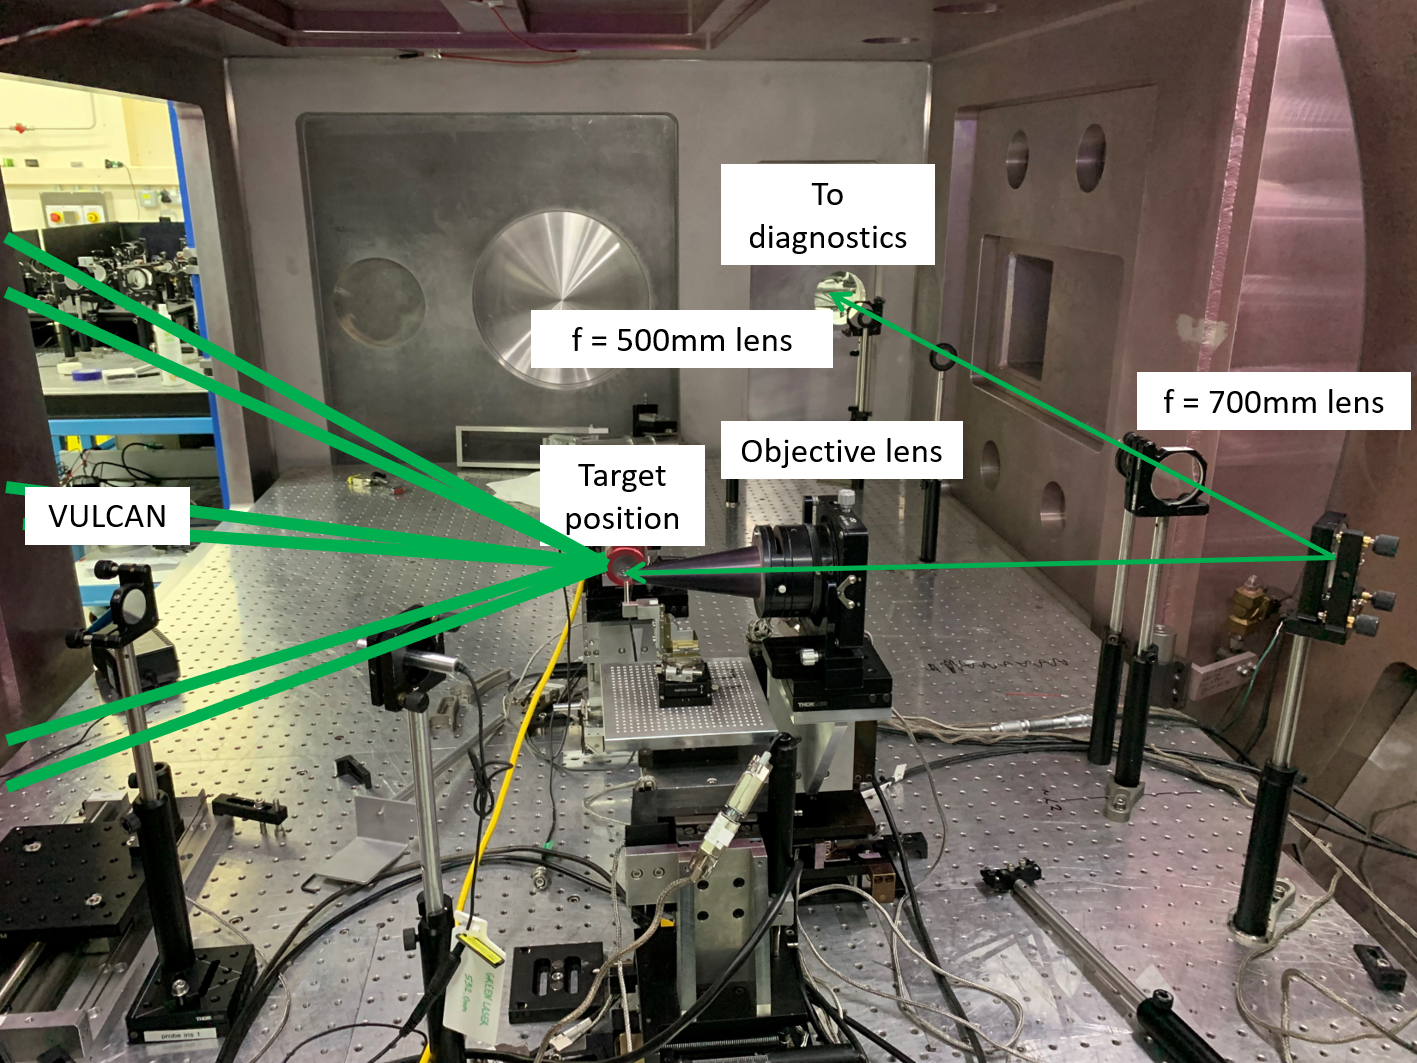
\includegraphics[width=1.0\textwidth]{figures/AppendixExperiment/InitialChamber.png}% Here is how to import EPS art
\caption{\label{fig:Appx-InitialChamber} The target chamber for the initial setup. The probe laser (thin green line) enters from the chamber window, and passes through the optics to the chamber windows. The reflected probe laser light and the self emission is captured by the objective lens and follows the same route back through the chamber window.}
\end{centering}
\end{figure}

\begin{figure}[ht]
\begin{centering}
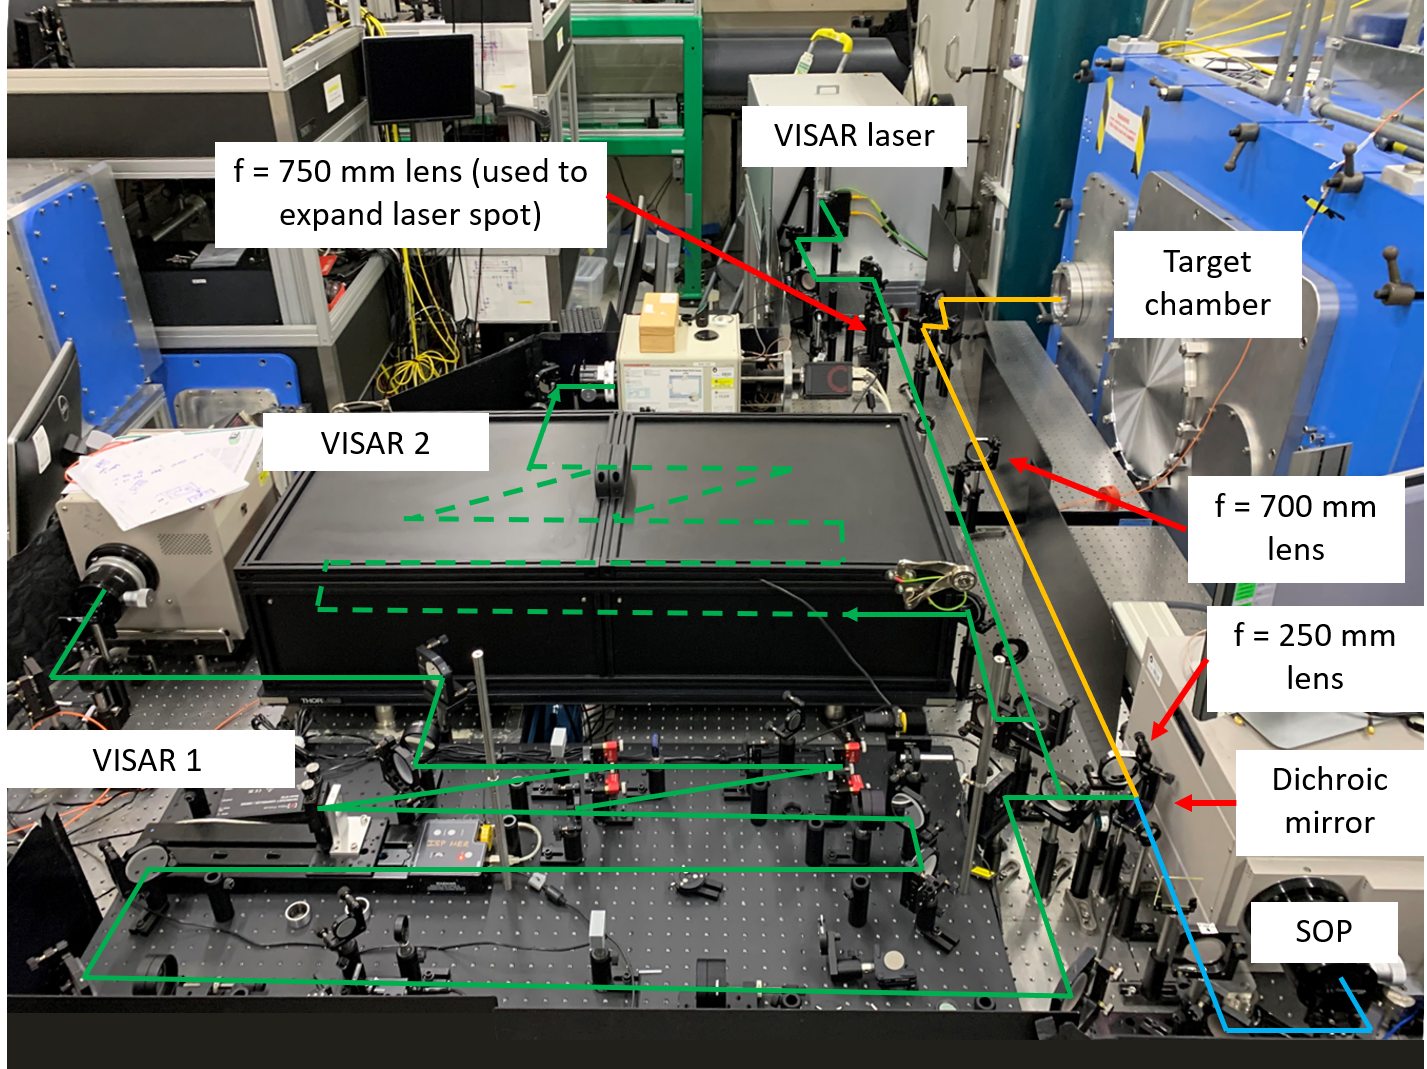
\includegraphics[width=1.0\textwidth]{figures/AppendixExperiment/InitialSetup.png}% Here is how to import EPS art
\caption{\label{fig:Appx-InitialSetup} The initial setup outside the target chamber. The light from the target travelling from the chamber is represented by the orange line. The dichroic mirror seperates the self-emission (blue) from the reflected probe laser (green). The self-emission continues onwards to the SOP streak, while the reflected probe laser goes to the two VISARs. The probe laser itself is injected into the beamsplitter at the second VISAR, and travels up through the beampath into the target chamber. A 750 mm lens is also shown, which was used to try and decollimate the probe laser prior to the setup being changed.}
\end{centering}
\end{figure}

\begin{figure}[ht]
\begin{centering}
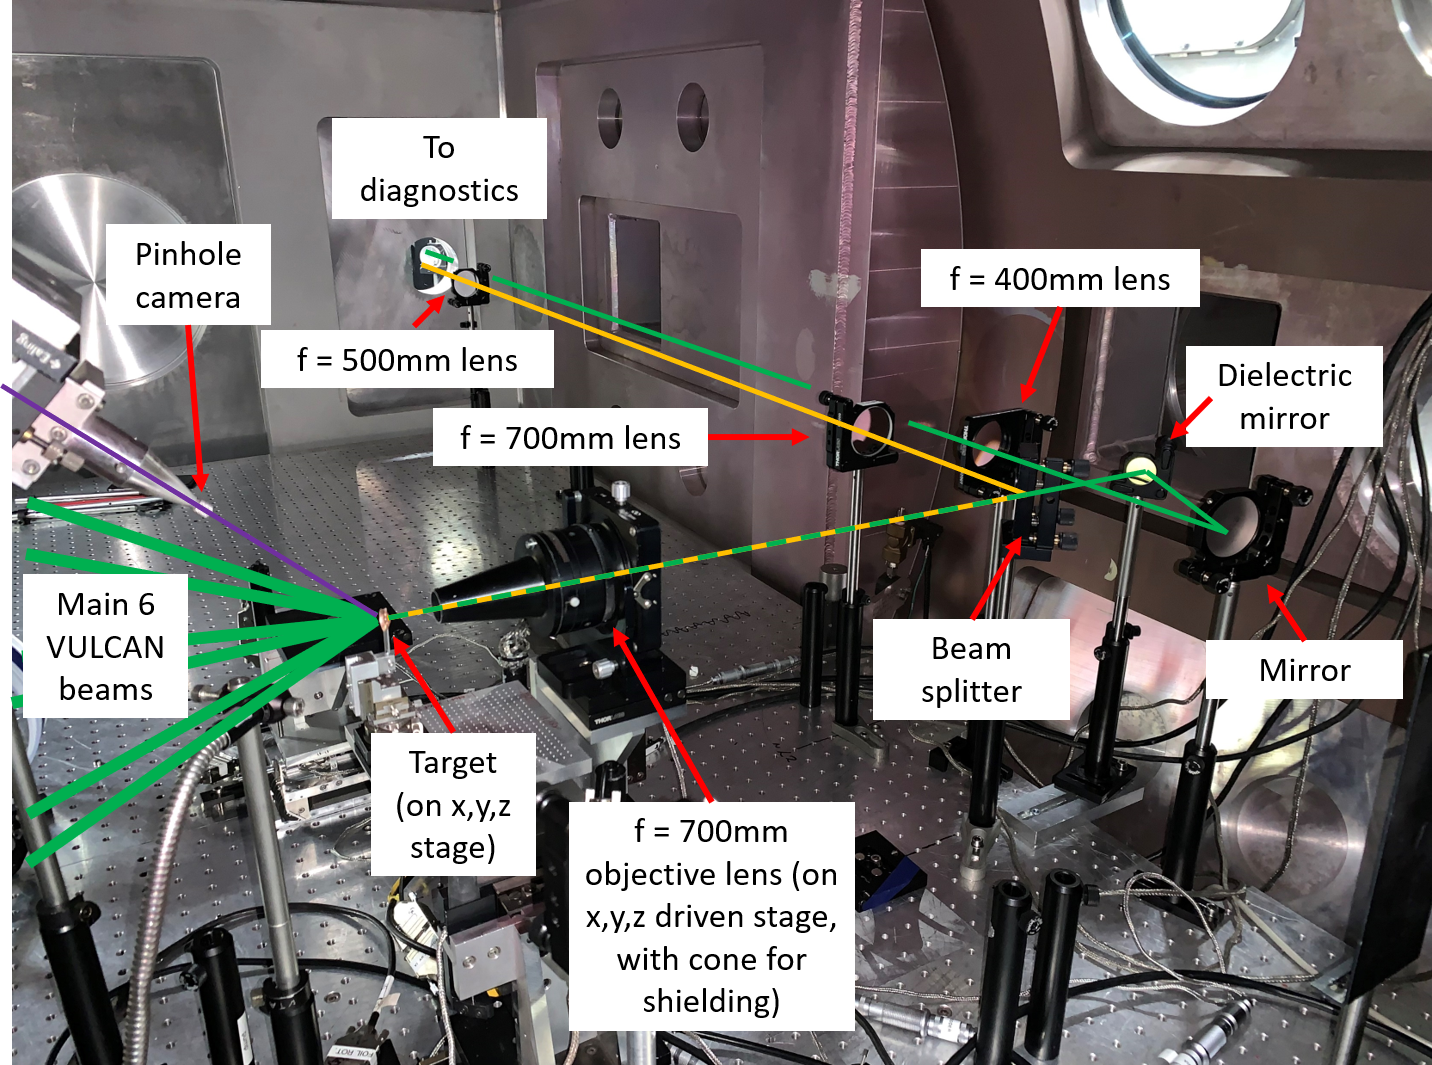
\includegraphics[width=1.0\textwidth]{figures/AppendixExperiment/FinalChamber.png}% Here is how to import EPS art
\caption{\label{fig:Appx-FinalChamber} The target chamber for the final setup. The probe laser beam path (green) is now separate from the imaging beam path (orange). The first mirror has been replaced with a beamsplitter, allowing the probe laser to be injected into the main path just prior to the objective lens (which now serves to collimate this beam). The objective lens captures the reflected probe light, plus the self-emission, and this is transmitted down the orange beam path and out of the chamber as in the initial setup. The pinhole camera is also shown in this image, with it's line of sight represented by the purple line. }
\end{centering}
\end{figure}

\begin{figure}[ht]
\begin{centering}
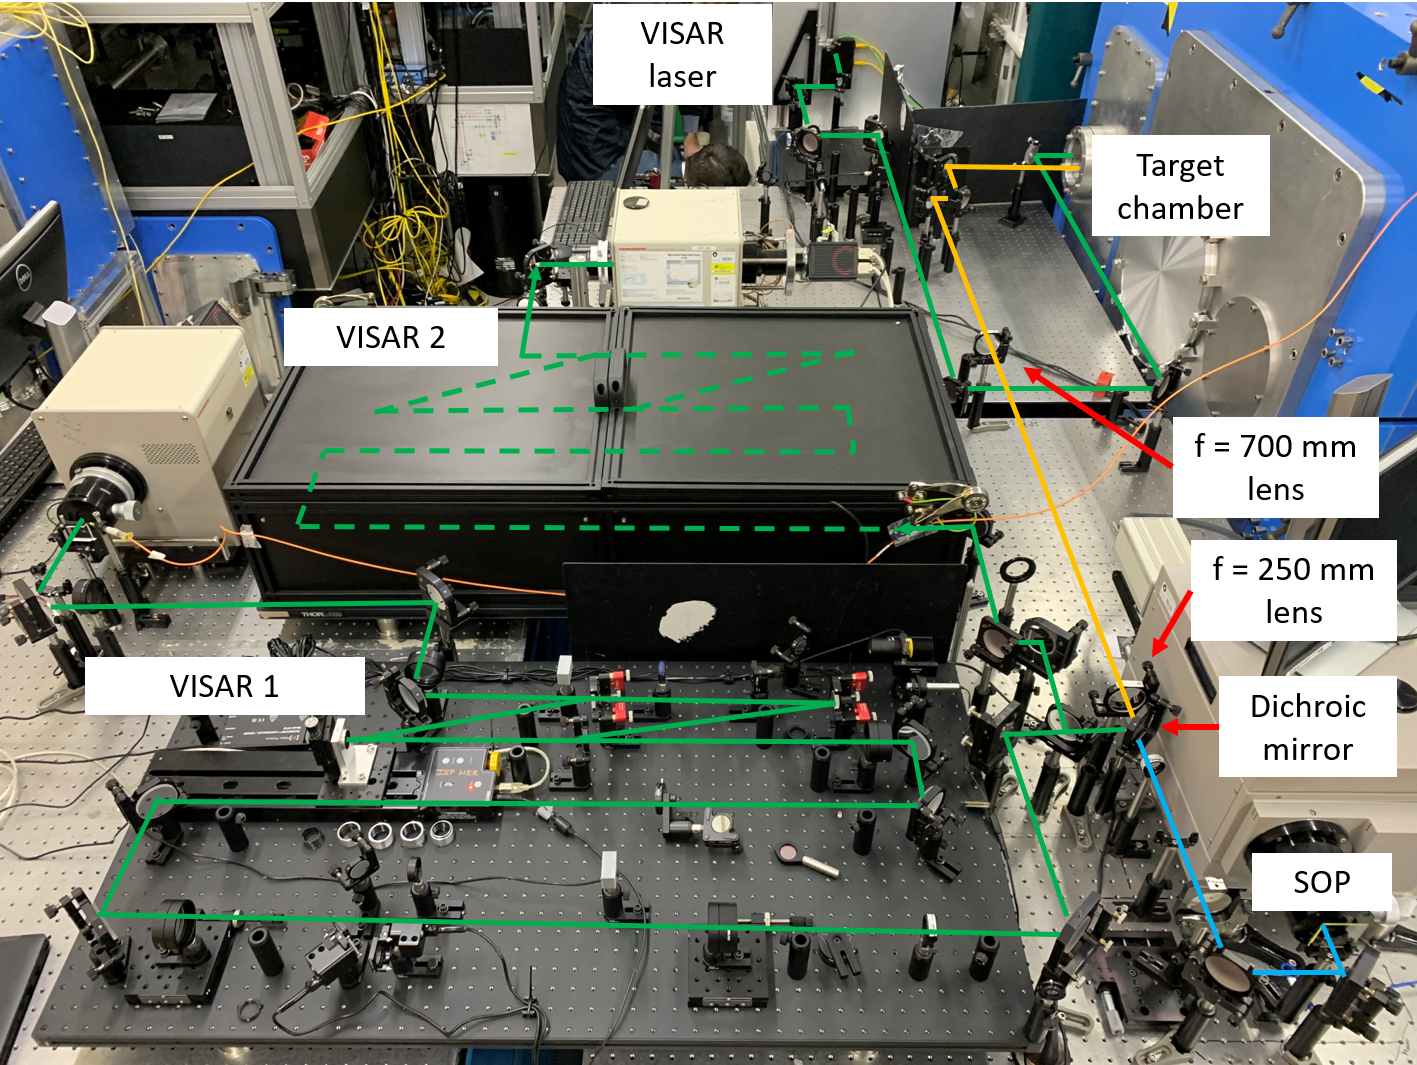
\includegraphics[width=1.0\textwidth]{figures/AppendixExperiment/FinalSetup.png}% Here is how to import EPS art
\caption{\label{fig:Appx-FinalSetup} The final setup outside of the chamber. The imaging beamlines are unchanged from before, except the beamsplitter before the second VISAR has been changed to a mirror. The probe laser follows a new route into the target chamber.}
\end{centering}
\end{figure}

\begin{figure}[ht]
\begin{centering}
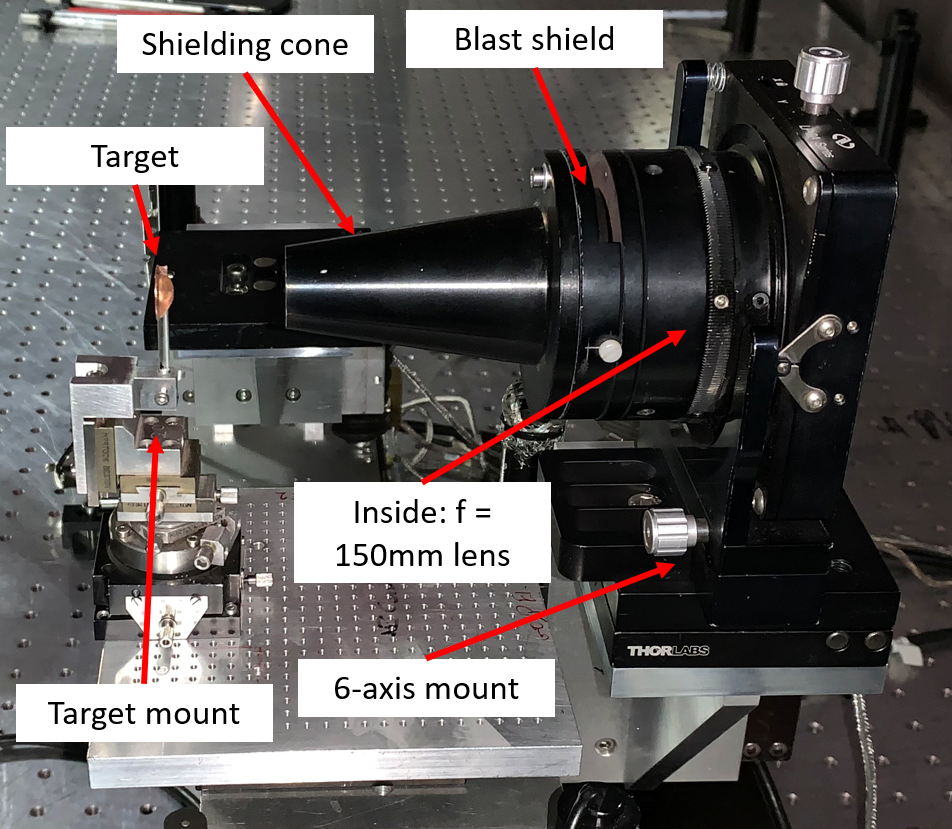
\includegraphics[width=1.0\textwidth]{figures/AppendixExperiment/ObjectiveLens.png}% Here is how to import EPS art
\caption{\label{fig:Appx-Objective} A close-up image showing the target and objective lens.}
\end{centering}
\end{figure}

\begin{figure}[ht]
\begin{centering}
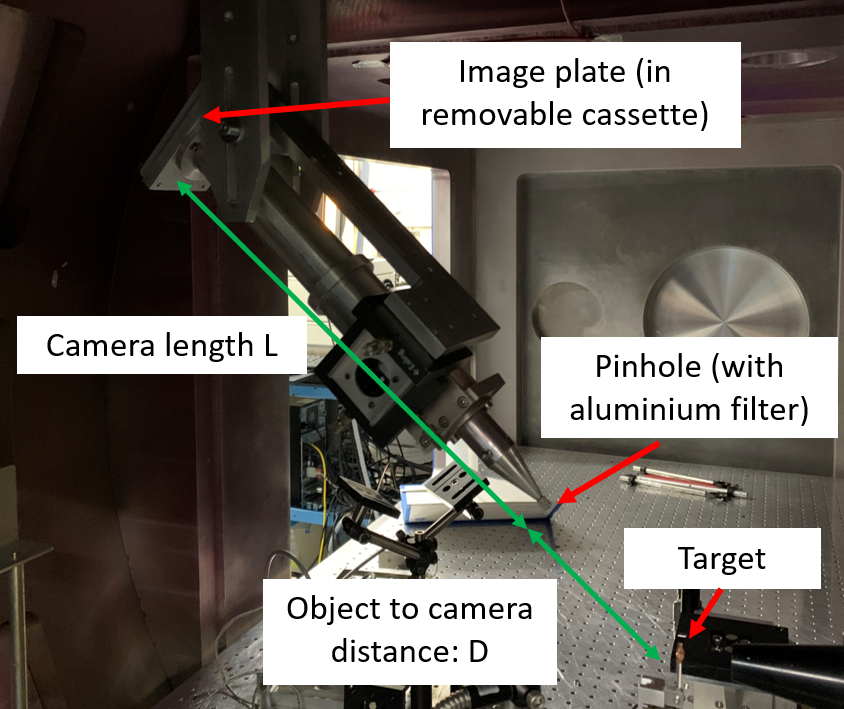
\includegraphics[width=1.0\textwidth]{figures/AppendixExperiment/Pinhole.png}% Here is how to import EPS art
\caption{\label{fig:Appx-Pinhole} The pinhole camera, in position. The image plate is placed at the rear of the camera. A thin piece of aluminium is placed on the front of the pinhole to provide filtering of low-energy x-rays. }
\end{centering}
\end{figure}

\begin{figure}[ht]
\begin{centering}
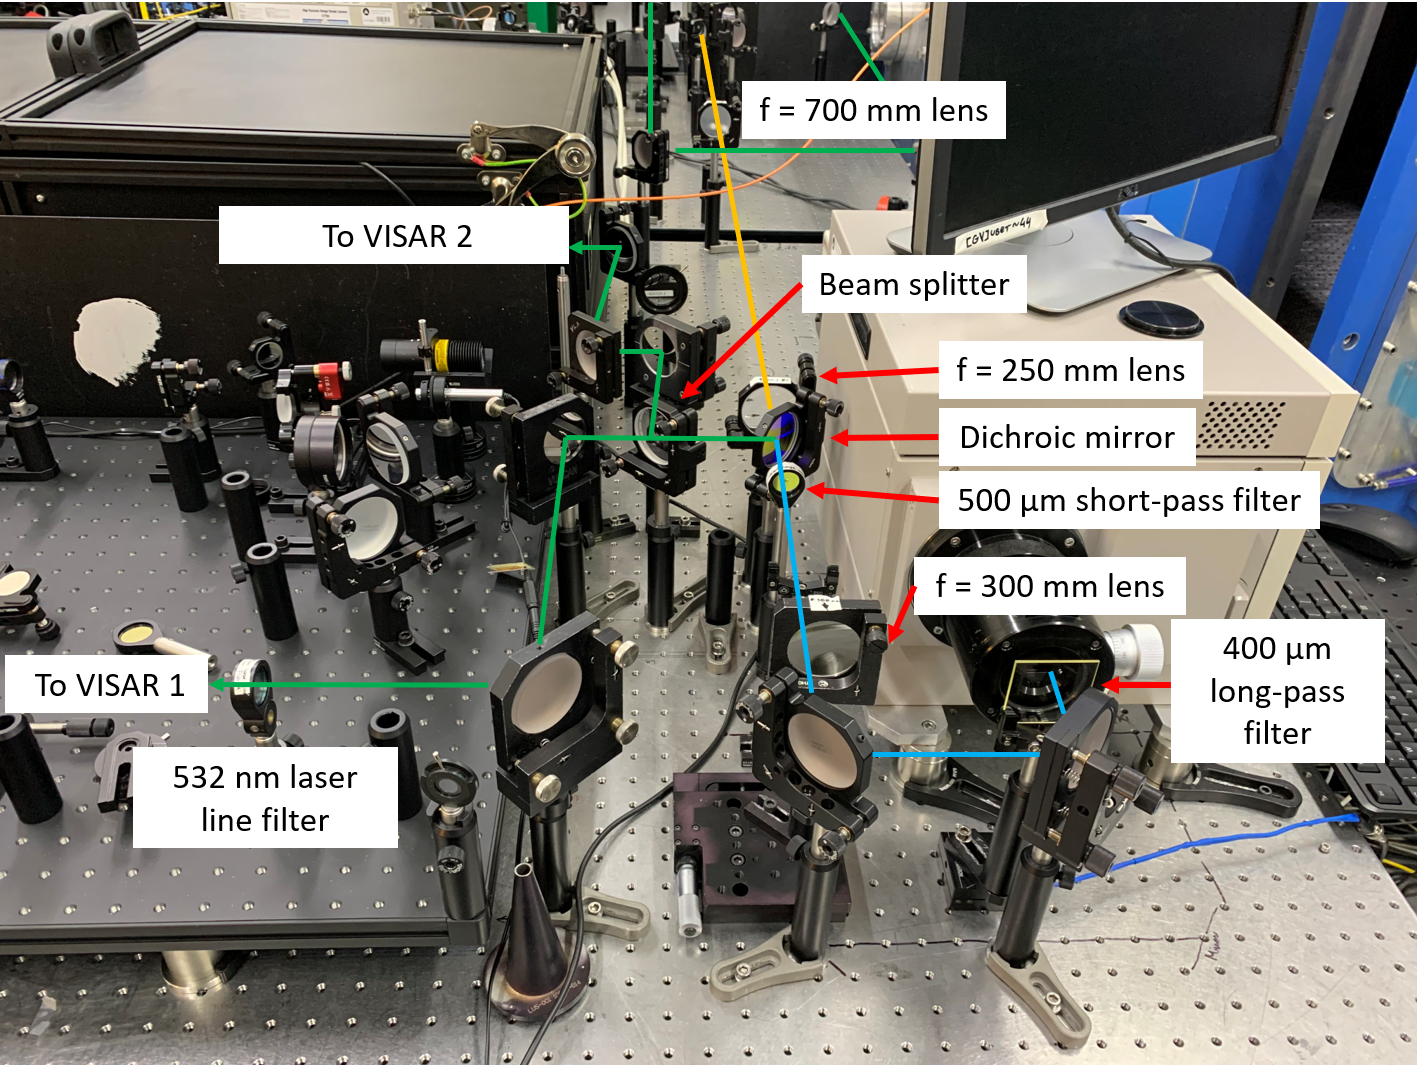
\includegraphics[width=1.0\textwidth]{figures/AppendixExperiment/DichroicCloseUp.png}% Here is how to import EPS art
\caption{\label{fig:Appx-Dichroic} A close-up image of the components around the dichroic mirror, showing the filters in position. The 400\unit{\micro\meter} long-pass filter is in a slightly different position to the main schematic; this change in position has no effect.}
\end{centering}
\end{figure}

\begin{figure}[ht]
\begin{centering}
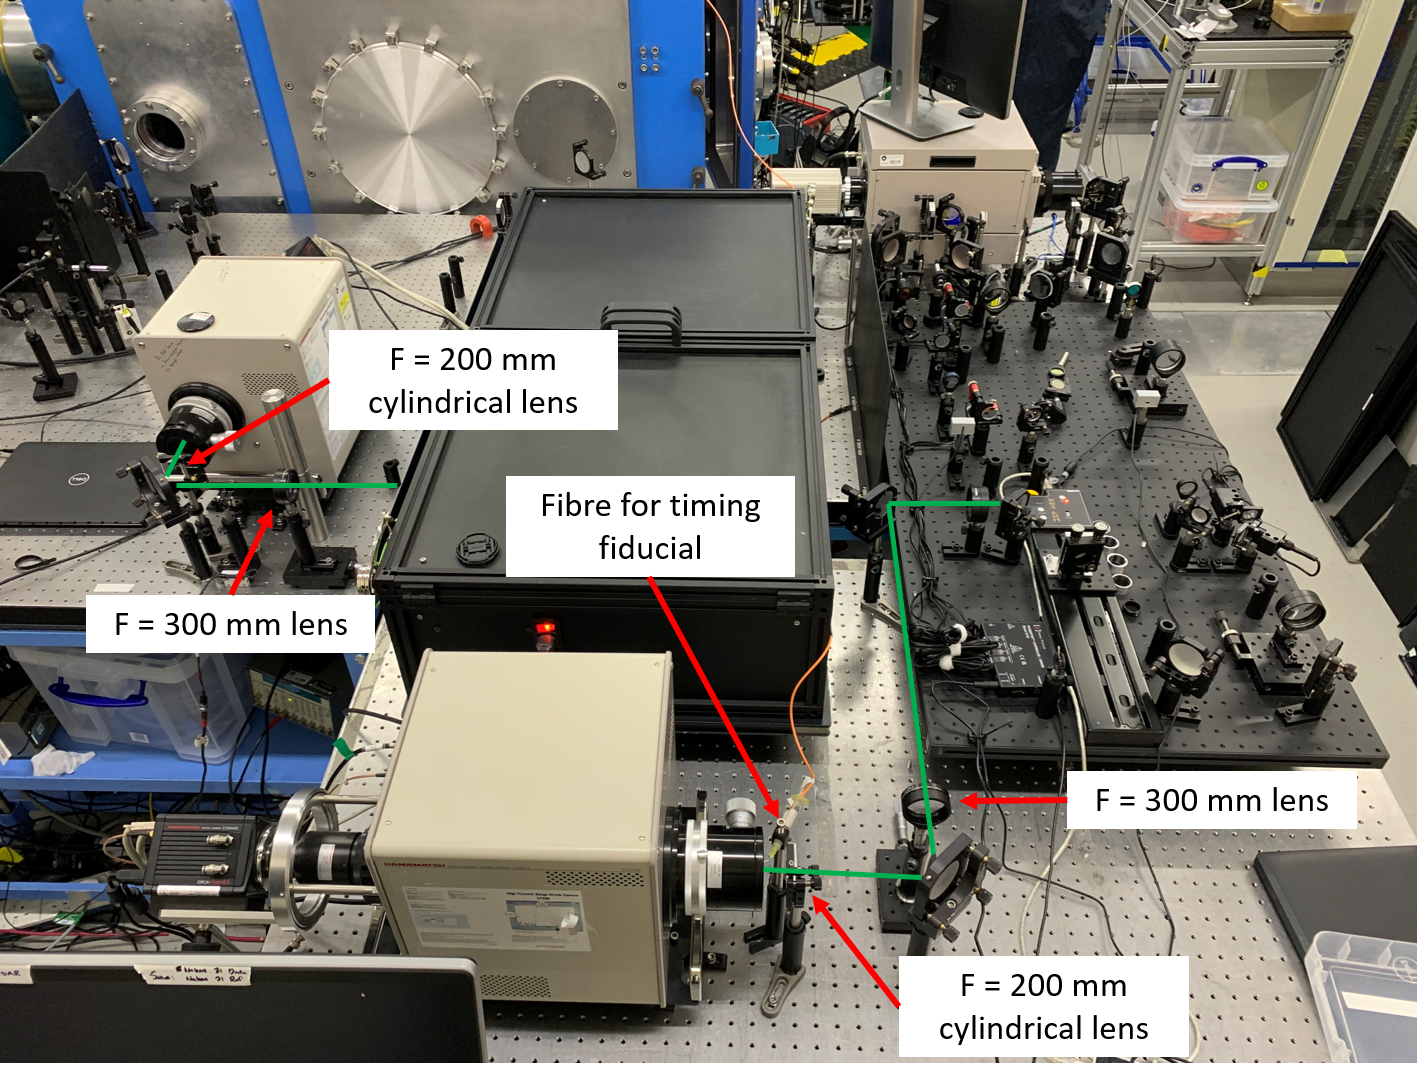
\includegraphics[width=1.0\textwidth]{figures/AppendixExperiment/VISARstreaks.png}% Here is how to import EPS art
\caption{\label{fig:Appx-VISARstreaks} A close up showing the beam path as the imaging lines leave the VISARs and are transmitted to the streak cameras. The fiducial captures light leaking through one of the VULCAN mirrors, and shines this on the side of one of the streak cameras.}
\end{centering}
\end{figure}

\begin{figure}[ht]
\begin{centering}
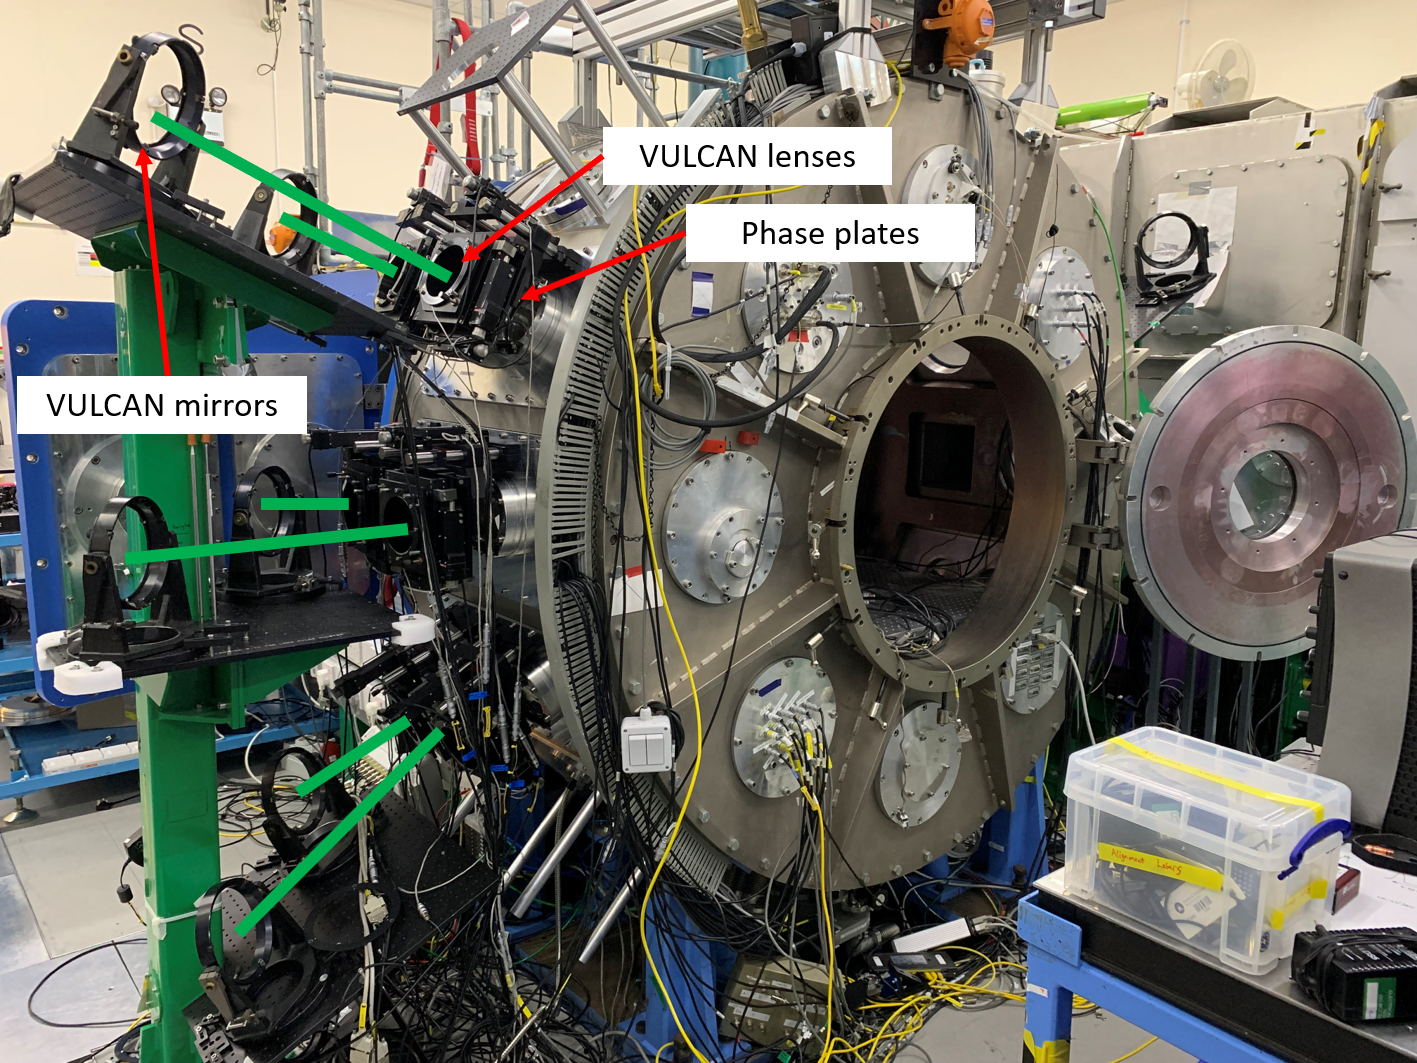
\includegraphics[width=1.0\textwidth]{figures/AppendixExperiment/Chamberandvulcan.png}% Here is how to import EPS art
\caption{\label{fig:Appx-Chamberandvulcan} The VULCAN target chamber, showing the VULCAN mirrors, lenses, and phase plates position. These beams enter through six ports on the chamber and irradiate the target. The two chamber doors are sealed shut so that the chamber can be pumped down to vacuum.}
\end{centering}
\end{figure}

\begin{figure}[ht]
\begin{centering}
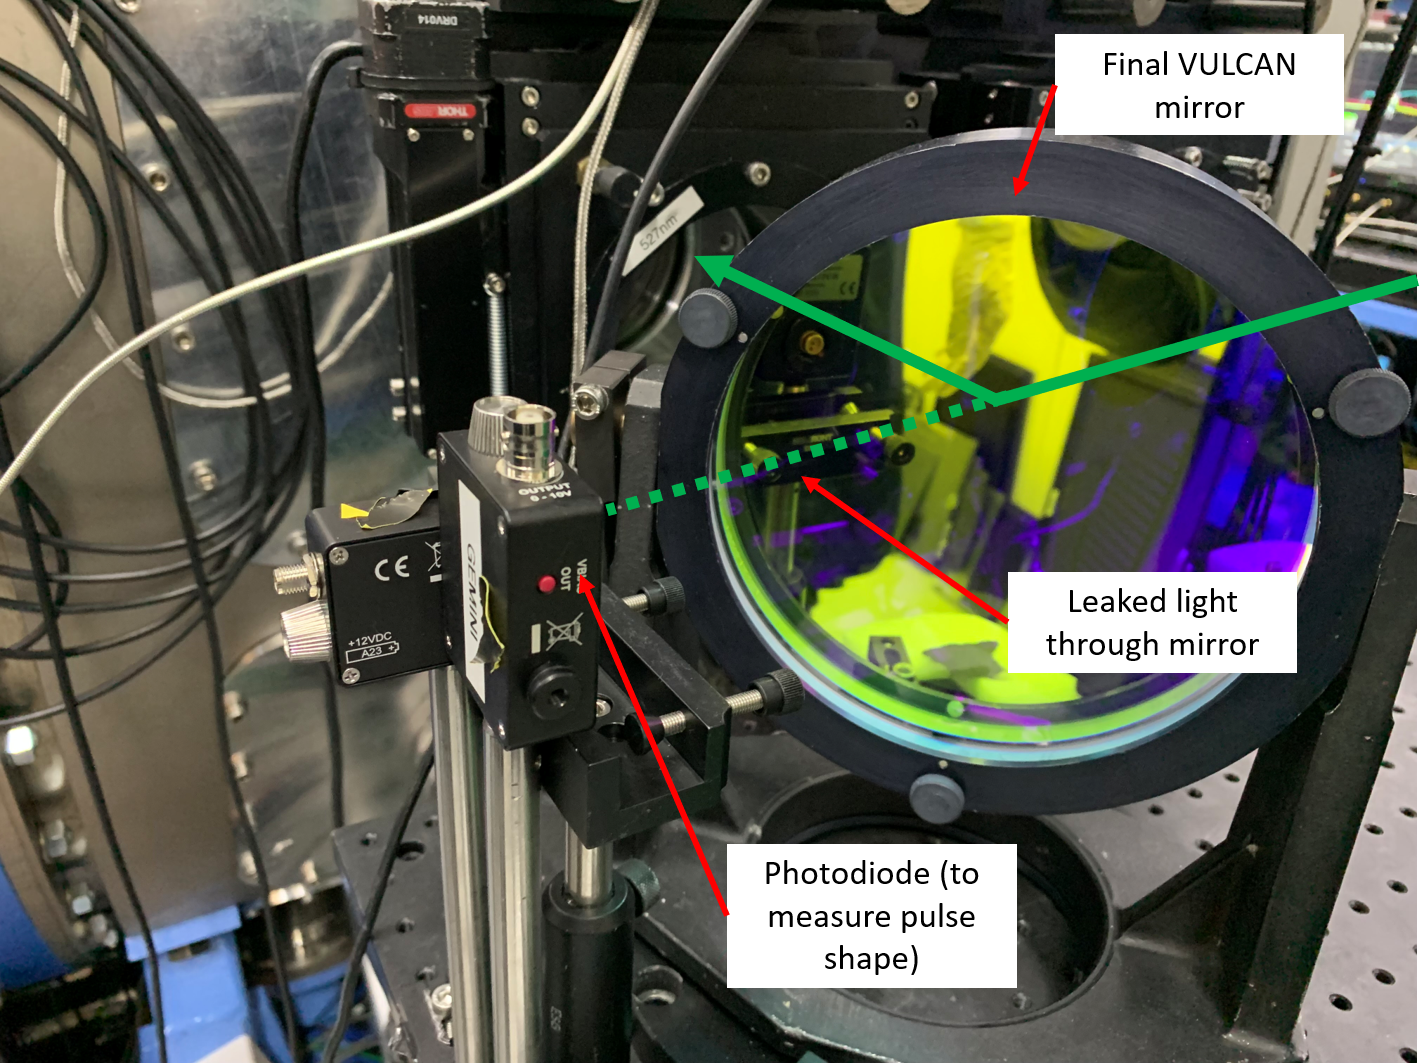
\includegraphics[width=1.0\textwidth]{figures/AppendixExperiment/Photodiode.png}% Here is how to import EPS art
\caption{\label{fig:Appx-Photodiode} A close up of one of the final VULCAN mirrors shown in Figure \ref{fig:Appx-Chamberandvulcan}. Each  of these mirrors has a small photodiode placed behind it. A small fraction of the VULCAN light leaks through the mirror, and this is detected by the photodiode and recorded to measure the pulse shape.}
\end{centering}
\end{figure}

\section{Target images}

The following images show the targets used in this experiment. With the exception of the first image, these were provided by Chris Spindloe and CLF target fabrication.

\begin{figure}[ht]
\begin{centering}
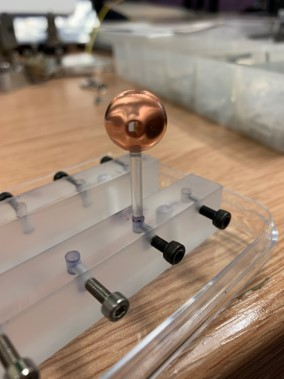
\includegraphics[width=1.0\textwidth]{figures/AppendixExperiment/Target.jpg}% Here is how to import EPS art
\caption{\label{fig:Appx-Target} A photograph of the target. It can be seen that half of the front is covered by foam (white), while the other half is quartz (as the quartz is transparent, this half appears gold due to the gold layer underneath).}
\end{centering}
\end{figure}

\begin{figure}[ht]
\begin{centering}
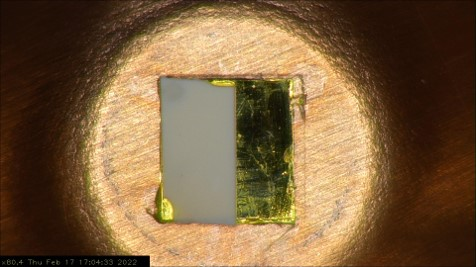
\includegraphics[width=1.0\textwidth]{figures/AppendixExperiment/TargetMicroscope.jpg}% Here is how to import EPS art
\caption{\label{fig:Appx-TargetMicroscope} Microscope image of a target, showing the step between the foam and quartz. }
\end{centering}
\end{figure}

\begin{figure}[ht]
\begin{centering}
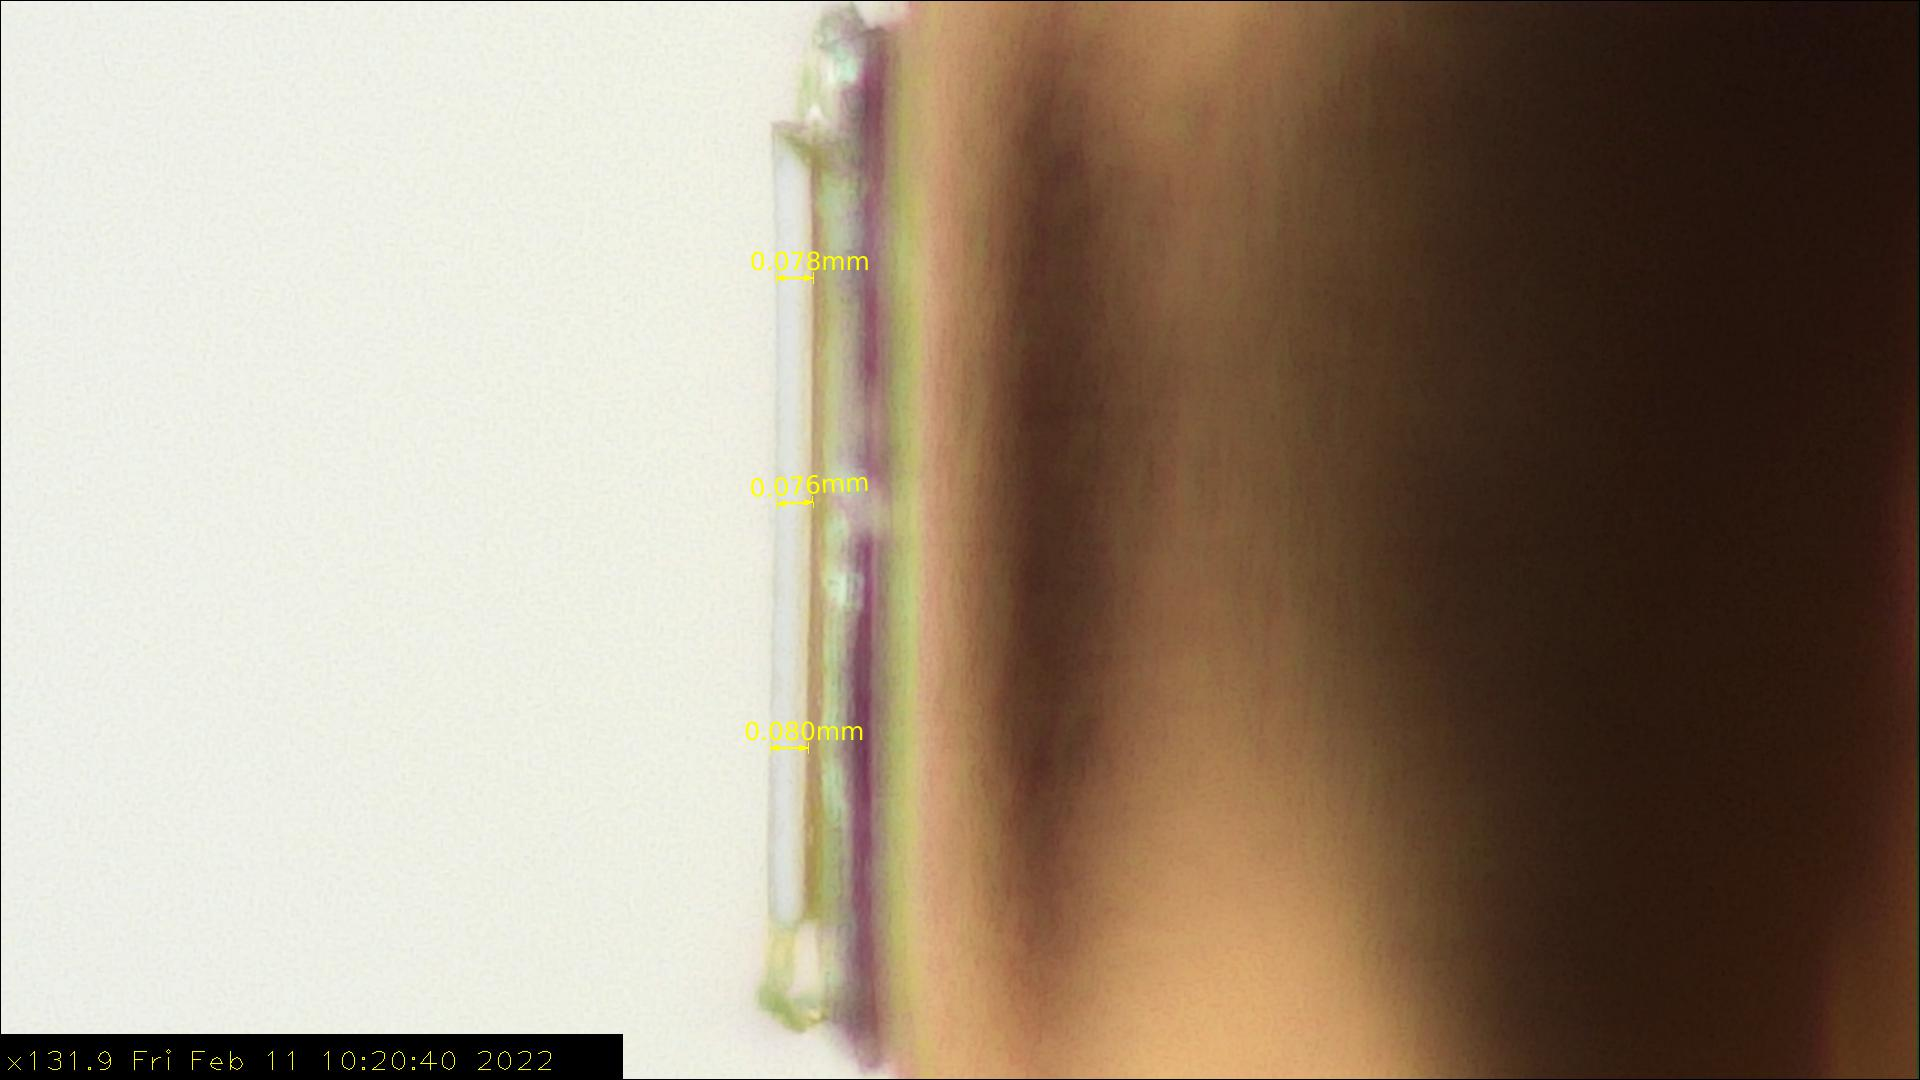
\includegraphics[width=1.0\textwidth]{figures/AppendixExperiment/TargetSideOn.jpg}% Here is how to import EPS art
\caption{\label{fig:TargetSideOn} Microscope image of the target, side on. The foam has been measured at three positions, providing the foam thickness used for the average velocity calculation. The variation between different points across a range of these images was used to estimate the uncertainty in this measurement.}
\end{centering}
\end{figure}

\begin{figure}[ht]
\begin{centering}
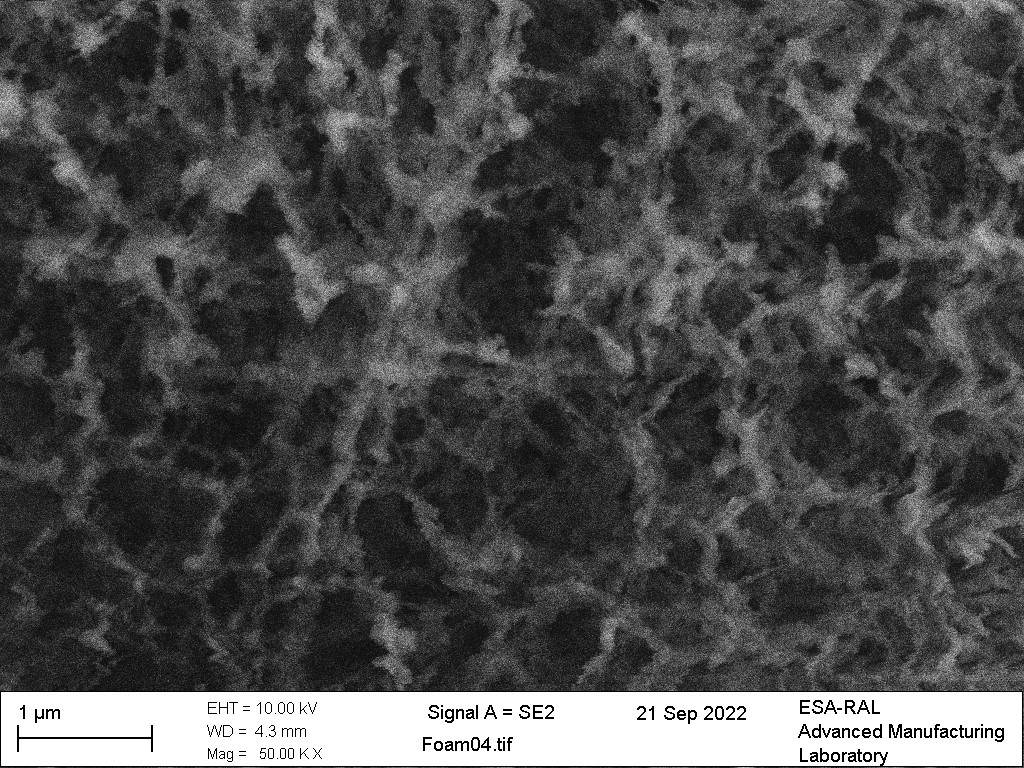
\includegraphics[width=1.0\textwidth]{figures/AppendixExperiment/FoamSEM.jpg}% Here is how to import EPS art
\caption{\label{fig:Appx-Foam04} A scanning electron microscope image of the foam material. Fibres of plastic polymer can be seen. A number of these were performed, and allowed the pore size to be estimated as roughly 1 \unit{\micro\meter}.}
\end{centering}
\end{figure}

\section{CAD models of experimental setup}

The following section shows a series of CAD models (and associated technical drawings) of the initial and final experimental setups. These were produced post-experiment, and feature the real positions of each of the components.

\begin{figure}[ht]
\begin{centering}
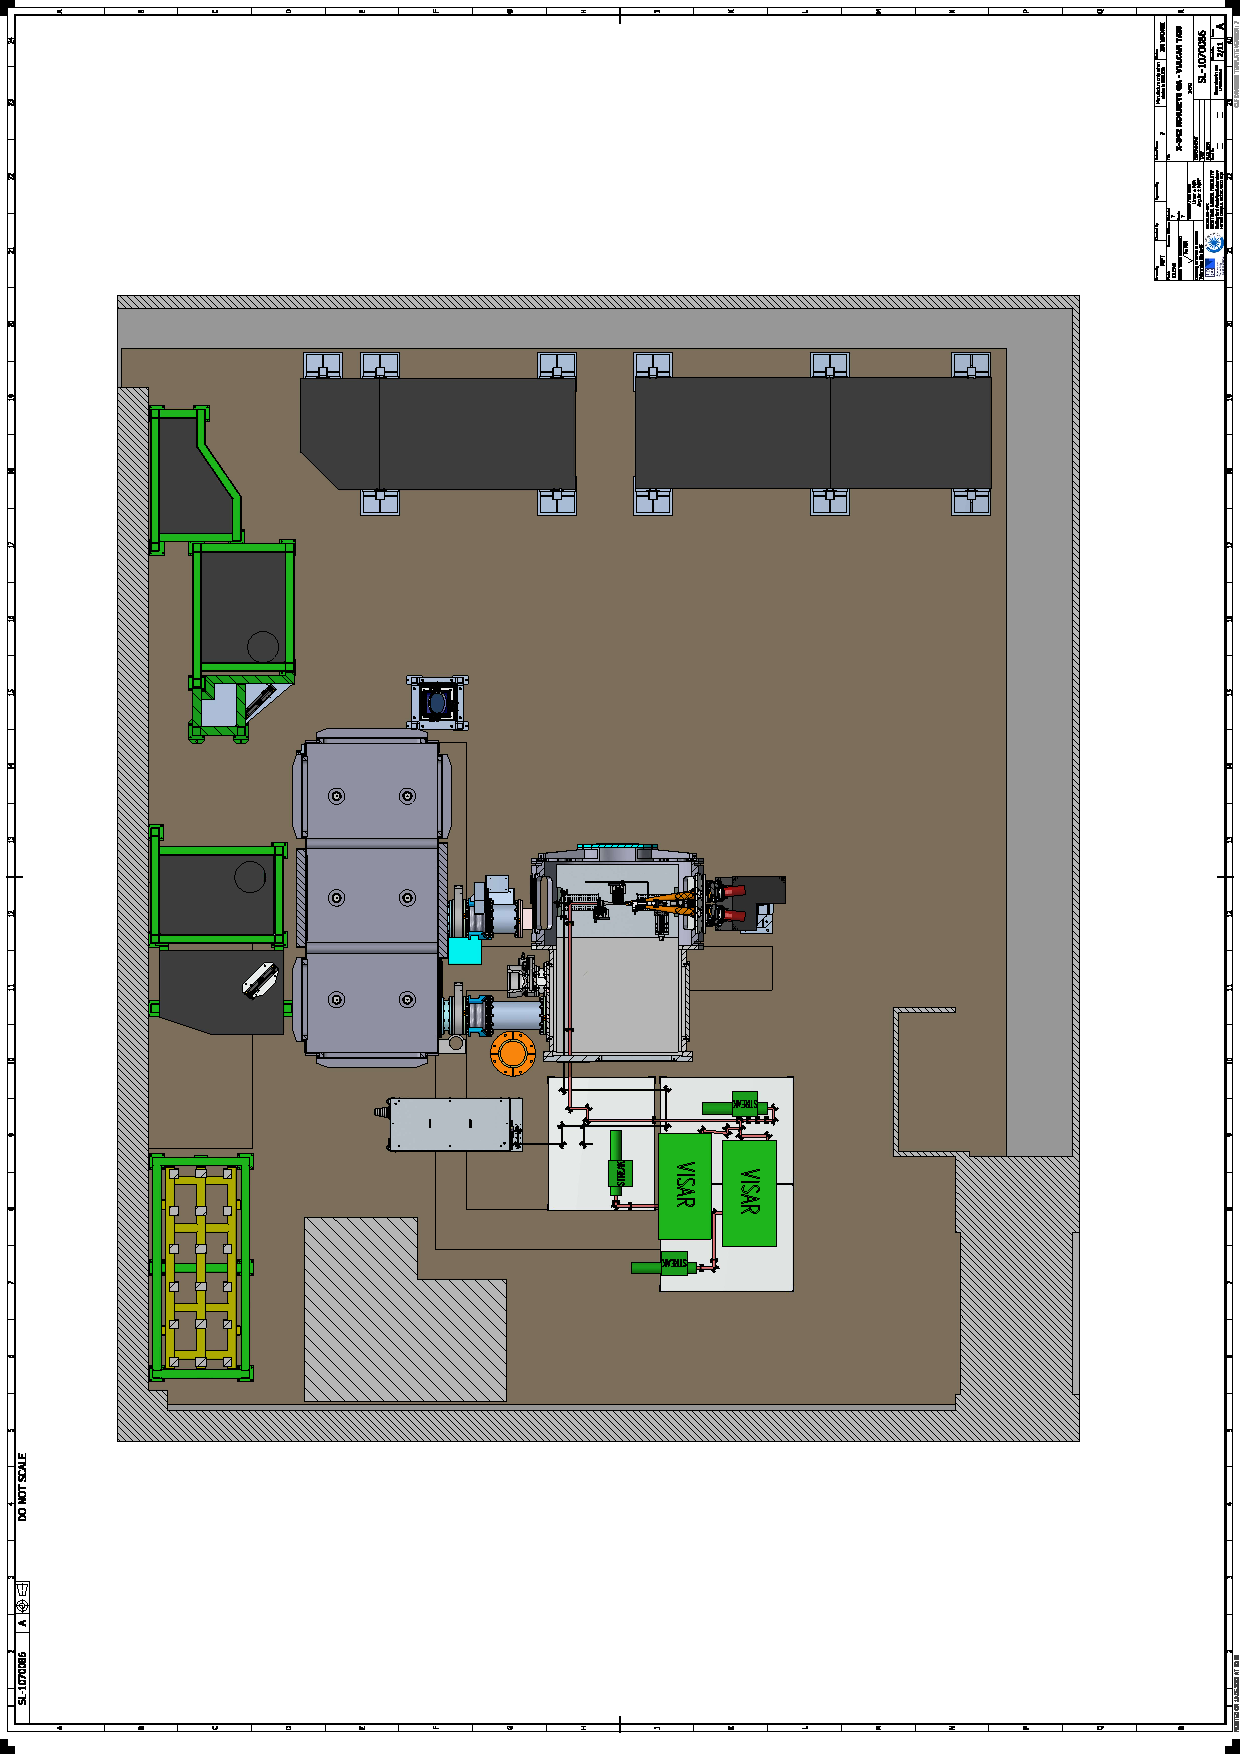
\includegraphics[width=1.0\textwidth]{figures/AppendixExperiment/CADTable3D.pdf}% Here is how to import EPS art
\caption{\label{fig:Appx-CADFinalSetup} 3D CAD model showing the final configuration used in the experiment}
\end{centering}
\end{figure}

\begin{figure}[ht]
\begin{centering}
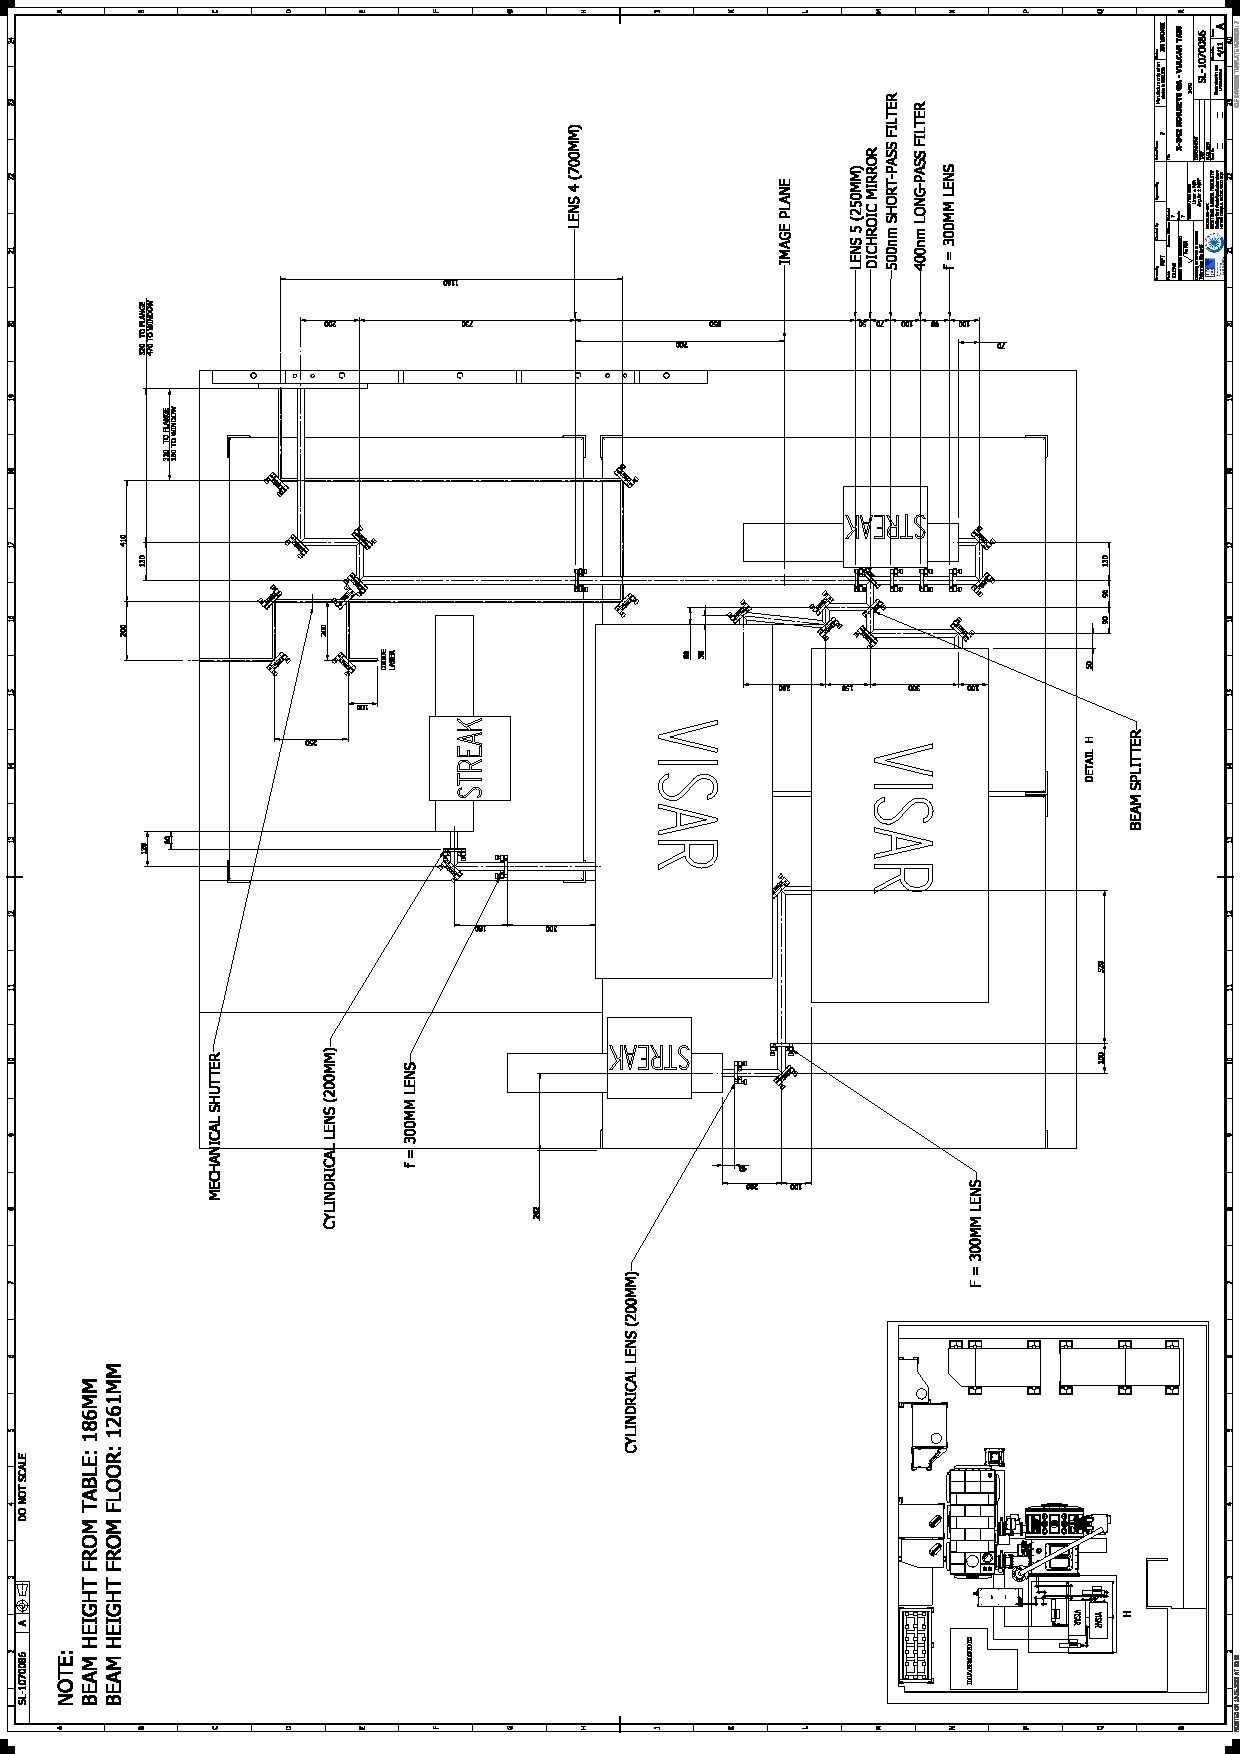
\includegraphics[width=1.0\textwidth]{figures/AppendixExperiment/CADFinalMeasured.pdf}% Here is how to import EPS art
\caption{\label{fig:Appx-CADFinalSetupMeasured} Engineering drawing showing the optical tables for the final setup, with full measurements.}
\end{centering}
\end{figure}


\begin{figure}[ht]
\begin{centering}
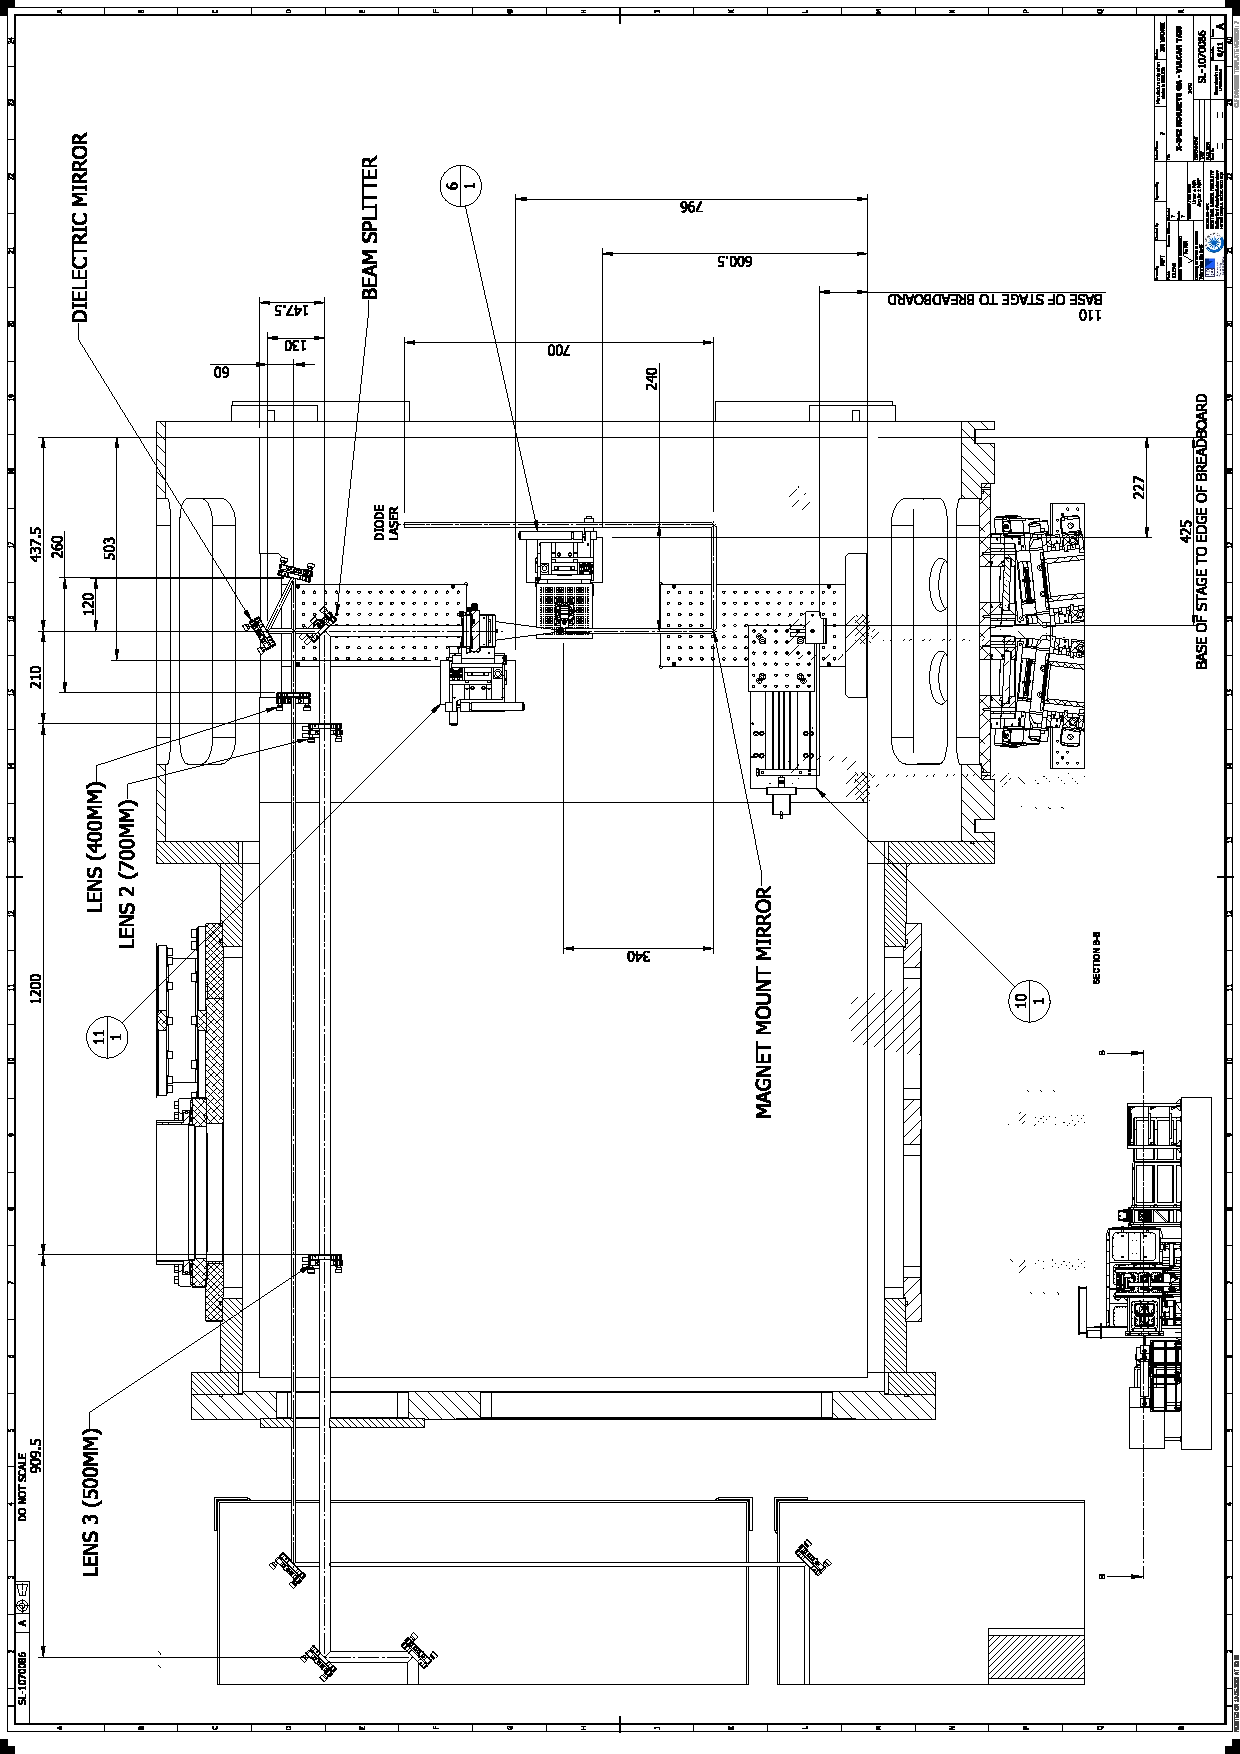
\includegraphics[width=1.0\textwidth]{figures/AppendixExperiment/CADFinalChamber.pdf}% Here is how to import EPS art
\caption{\label{fig:Appx-CADFinalChamberMeasured} Engineering drawing showing the target chamber for the final setup, with full measurements.}
\end{centering}
\end{figure}